\NeedsTeXFormat{LaTeX2e}
\documentclass[11pt,a4paper]{article}
\usepackage{latexsym}
\usepackage{epsfig}
\usepackage{graphicx}
\usepackage{amsmath}
%\usepackage{listings}
\usepackage{verbatim}
\usepackage{amssymb}
\usepackage{hyperref}
\usepackage{listings} 

\author{A. Studer, Scientific Computing, PSI}
\title{Pair correlation function of a liquid}


\begin{document}
\maketitle

\begin{abstract}
A short discussion about the pair correlation of a fluid is given. Ideally the following summary
helps to understand in a self contained way how the pair correlation function is defined, measured and calculated.
\end{abstract}



\section{Theoretical Considerations}
\subsection{Definition of the pair correlation and Ornstein Zernike equation}
The Ornstein Zernike equation aims at finding the pair correlation function $g(\vec r)$, which basically
describes the probability to find two arbitrary particles in the fluid at a relative distance $\vec r$. 
If the fluid is isotropic, then $g(\vec r) = g(r)$ and $g(r)$ is also called the radial distribution function. 
It is intuitively clear that there is a short range order in a liquid, meaning that molecules gather in shells around a test particle
and hence the pair correlation function is somehow oscillating (until this short range order vanishes). How exactly this
oscillation looks like is analyzed in the following.

\begin{minipage}[hbt]{5cm}
	\centering
	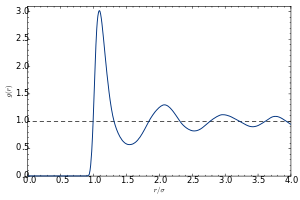
\includegraphics[width=5cm]{RDF.png}
	\label{"halllo"}
\end{minipage}
\hfill
\begin{minipage}[hbt]{5cm}
	\centering
	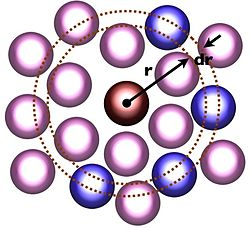
\includegraphics[width=5cm]{RDF_illustrated.png}
	\label{Bild2}
\end{minipage}
\newline
\textit{Figure 1: pair correlation function and its illustration with molecules} \newline \newline
The 'first-principle-way' to calculate the pair correlation function is to use the framework of (classical) statistical mechanics:
Suppose that $N$ identical particles are gathered in a box of volume $V$ which is thermally connected to a heat bath at temperature $T$. 
Then the probability density $f$ to find the $N$ particles at positions $\vec r_1, \dots \vec r_n$ is given by the canonical ensemble

\begin{equation}
f(\vec r_1, \dots \vec r_n) = \frac{1}{Z_N} e^{-\beta U(\vec r_1, \dots \vec r_n)}
\end{equation}
where $U$ is the total potential energy of the particles and $\beta = 1/k_BT$. (The momentum part of the phase space is already 'integrated out'.
Furthermore, we claim that there is no external potential such that $U$ only contains internal particle interactions which leads to a
homogeneous particle density).
$Z_N$ is a normalization constant such that

\begin{equation}
\int f(\vec r_1, \dots \vec r_n)d \vec r_1 \dots d\vec r_n = 1
\end{equation}
(The molecules are for sure somewhere. Although $Z_N$ plays an important role in statistical mechanics, it is not that relevant inhere).\newline
The basic step to calculate the pair correlation function, say between particle 1 and 2, is to calculate
\begin{equation}
\int f(\vec r_1, \vec r_2,\vec r_3,\dots \vec r_n)d \vec r_3 \dots d\vec r_n
\end{equation}
The integral expresses the idea that we simply don't bother where the other molecules are. \newline
The pair correlation function is supposed to describe the probability that the particles 1 and 2 are at a distance $\vec r$,
which is close to  the definition of the 2 particle density:

\begin{equation}
\rho_{12}^{(2)} (\vec r) = \frac{1}{V}
\int f(\vec r_1, \vec r_1 + \vec r,\vec r_3,\dots \vec r_n) d\vec r_1 d\vec r_3 \dots d\vec r_n
\end{equation}

where we also integrate over $\vec r_1$, since the absolute position of this particle does not matter. The above definition is the two particle
density induced by particle 1 and 2; but generally, one is interested in the particle density induced by all particle pairs (or analogously: the
pair distribution function for \textit{any} pair of particles). Since there are $N(N-1)$ particle pairs in a fluid of $N$ (identical) particles
and since the fluid assumed to be homogeneous \footnote{All particle pairs are equal with respect to relative distance (on average).}
, we define

\begin{equation}
\rho^{(2)} (\vec r) = \frac{N(N-1)}{V} \int f(\vec r_1, \vec r_1 + \vec r,\vec r_3,\dots \vec r_n) d\vec r_1 d\vec r_3 \dots d\vec r_n
\end{equation}

The pair density is now normalized with respect to the ideal gas density
\footnote{The ideal gas is interaction- and hence correlation-free. Its constituent are volume-less particles. The normalization
is such that the pair correlation function of an ideal gas $\rightarrow 1$ for $N$ large.}.
This finally yields the definition of the pair distribution function

\begin{equation}
g(\vec r) = \rho^{(2)} (\vec r)/ \rho_{ideal}^{(2)} =
\frac{N(N-1)}{\rho^2 V} \frac{1}{Z_N}\int e^{-\beta U(\vec r_1, \vec r_1 + \vec r,\vec r_3,\dots \vec r_n)} d\vec r_1 d\vec r_3 \dots d\vec r_n
\end{equation}

where $\rho = N/V$ is the average particle number density. $\rho_V \in [0, \dots, 0.74]$, where $\simeq 0.74$ is the maximal close packaging 
density for equal spheres. (This state may only be reached close to the phase transition to the frozen sate).
The fluid is assumed homogeneous and hence of constant macroscopic density. ($\rho^2$ is the two pair density of a ideal fluid, 
since an uncorrelated pair density is simply the product of the two single particle densities, i.e the probability to find a particle at position $r_1$
and another one at position $r_2$ is simply the product of the probabilities of these disjoint events to happen).\newline
The practical problem with the above integral is that for a realistic particle number it is extremely high dimensional, which makes it intractable for
e.g. Monte Carlo integration. (Besides being hopeless to calculate analytically in most cases). This is where the Ornstein Zernike equation comes
into play: The OZ equation reduces the $3N$ problem to a 3 dimensional problem \footnote{Similar to density functional theory, where the 3$N$
dimensional wave function is substituted by a 3 dimensional density function.} 
The Ornstein Zernike equation reads

\begin{equation}
h(\vec r) = c(\vec r) + \rho (h*c) (\vec r)
\end{equation}
where $h(\vec r)$ is connected to the pair distribution function via $h(\vec r) = g(\vec r) -1$ and $c(\vec r)$ is a new function. (So we need an additional equation
where $c$ is involved to solve the OZ equation). In words, $c$ is a function which aims at taking into account the direct contributions to the pair correlation
function, whereas the convolution $h*c$ takes indirect contributions into account. (Say particle 1 and 2 interact directly via a potential term $V(\vec r_1, \vec r_2)$, this
would be responsible for the direct contribution. The relative position between particle 1 and 2 may also be influenced by a third particle (labeled 3),
which influences particle 1 via $V(\vec r_1, \vec r_3)$ and then in turn particle 2 via $V(\vec r_3, \vec r_2)$. So overall particle 3 mediates the distance between particle 1 and 2,
this is described by the term $h*c$). \newline Trying to formulate this idea in mathematical terms, we set

\begin{equation}
c(\vec r) = g_{total}(\vec r) - g_{indirect} (\vec r)
\end{equation}

So $c$ defined as the difference between total and indirect correlations should encompass the left-over direct contributions. $g_{total}(\vec r)$ is simply
$g^{(2)}(\vec r)$, the full pair correlation function. Before we proceed to define $g_{indirect}$. We proof that the total pair correlation can be written
in terms of the two-particle potential of mean force

\begin{equation}
g^{(2)}(\vec r_1, \vec r_2) = e^{- \beta w^{(2)} (\vec r_1, \vec r_2)  }
\end{equation}

where $w^{(2)}$ is defined by its gradient as
\begin{equation}
\nabla_i w^{(2)}(\vec r_1, \vec r_2) = 
\frac{ \int e^{-\beta U(\vec r_1, \dots \vec r_n)} (\nabla_i U) \, d\vec r_3 \dots d\vec r_n } 
     { \int e^{-\beta U(\vec r_1, \dots \vec r_n)}              \, d\vec r_3 \dots d\vec r_n }
\quad i = 1,2
\end{equation}
The idea of this definition is analogous the the pair correlation: The right hand side of the above equation equals the average
total force acting on particle 1 or 2 (or acting between 1 and 2), where the average is taken over all particle coordinates $>2$,
such that $w^{(2)}(\vec r_1, \vec r_2)$ can be seen as the remaining mean pair potential between particle 1 and 2.\newline
To proof equation (9), we first write it as
\begin{equation}
- \beta^{-1} \ln g^{(2)} = w^{(2)}
\end{equation}
hence the mean 1-2 force can be written as

\begin{equation}
\nabla_i w^{(2)}(\vec r_1, \vec r_2) =
- \beta^{-1} \frac{1}{g^{(2)} } \nabla_i \frac{1}{\tilde Z_n} \int e^{-\beta U(\vec r_1, \dots \vec r_n)}\, d\vec r_3 \dots d\vec r_n
\end{equation}

since $i=1,2$ and since the integral is over particle coordinates $>2$, the gradient can be moved inside the integral to yield

\begin{equation}
\nabla_i w^{(2)}(\vec r_1, \vec r_2) =
- \beta^{-1} \frac{1}{g^{(2)} } \frac{1}{\tilde Z_n} \int e^{-\beta U(\vec r_1, \dots \vec r_n)} (-\beta \nabla_i U) \, d\vec r_3 \dots d\vec r_n
\end{equation}

The $-\beta$ cancels, and since $1/g^{(2)}  = \tilde Z_n / \int e^{-\beta U(\vec r_1, \dots \vec r_n)}\, d\vec r_3 \dots d\vec r_n$
we recover equation (10) and hence equation (9) indeed holds.\newline If the potential is pairwise additive, 
$U(\{\vec r_i\}) = \sum_{i \ne j} u(\vec r_i, \vec r_j)$ , then for diluted gases
\begin{equation}
g^{(2)}(\vec r_1, \vec r_2) \rightarrow e^{- \beta u(\vec r_1, \vec r_2)  }
\quad
\rho \rightarrow 0
\end{equation}
This is due to $\nabla_i w^{(2)}(\vec r_1, \vec r_2) = \nabla_i u(\vec r_1, \vec r_2) + R$ where the rest terms $R$ tend to zero since
they all describe average inter-particle forces which go to zero for small densities.\newline
Now we are prepared to come back to the definition of $g_{indirect} (\vec r)$. Inspired by equation (9) and (14), we approximate the indirect
contribution via the indirect potential (which analogously is the total potential minus the direct potential)
\begin{equation}
g_{indirect} (\vec r_1, \vec r_2) = e^{- \beta [w^{(2)}(\vec r_1, \vec r_2)  - u(\vec r_1, \vec r_2) ] }
\end{equation}

Hence equation (8) becomes (for a potential which only depends on relative distances $\vec r = \vec r_1 - \vec r_2$)
\begin{equation}
c(\vec r) = g^{(2)}(\vec r) - e^{- \beta [w^{(2)}(\vec r)  - u(\vec r) ] } =
g^{(2)}(\vec r) - g^{(2)}(\vec r) e^{\beta u(\vec r) }
\end{equation}

Dropping the (2) index and defining $\Gamma(\vec r) = h(\vec r) - c(\vec r) = g(\vec r) -1 - c(\vec r)$

\begin{equation}
g(\vec r) = e^{- \beta u(\vec r) }(g(\vec r) - c(\vec r)) =
e^{- \beta u(\vec r) }(\Gamma(\vec r) + 1)
\end{equation}

The above is the so called Percus-Yevick Closure, an additional equation needed to solve the Ornstein-Zernike equation. Another famous closure
is the Hypernetted Chain Closure, which is derived by expanding the 'indirect' exponential in equation (15) to first order:

\begin{equation}
c(\vec r) = g(\vec r) -
(1 - \beta [w^{(2)}(\vec r)  - u(\vec r) ]) =
h(\vec r) - \beta u(\vec r) -\ln g(\vec r)
\end{equation}

some algebra yields the HNC closure
\begin{equation}
g(\vec r) = e^{- \beta u(\vec r) + \Gamma(\vec r) }
\end{equation}

Expanding $e^{\Gamma(\vec r) }$ in HNC to first order Taylor gives back PY closure, as expected.\newline
Since the justification of the OZ equation and its closures are a bit ad hoc (at least they were to me..) we repeat here the
idea by explicitly calculating the pair correlation function for a three particle system. (This is the minimum particle
number for the OZ idea to work). For three particles, and a pairwise additive potential there is
\begin{equation}
g(\vec r) = \frac{6}{\rho^2 V}\frac{1}{Z_3} \int
e^{- \beta u(\vec r_1, \vec r_1 + \vec r) }
e^{- \beta u(\vec r_1, \vec r_3) }
e^{- \beta u(\vec r_1 + \vec r, \vec r_3) }
\,
d\vec r_1
d\vec r_3
\end{equation}
If the two particle potential depends only on the modulus of the relative particle distance

\begin{equation}
g(\vec r) = \frac{6}{\rho^2 V}\frac{1}{Z_3} \int \int
e^{- \beta u( \vec r) }
e^{- \beta u(\vec r_3 - \vec r_1) }
e^{- \beta u(\vec r_3 - \vec r_1 - \vec r) }
\,
d\vec r_1
d\vec r_3
\end{equation}
Hence

\begin{equation}
g(\vec r) = e^{- \beta u( \vec r) }
\frac{6}{\rho^2 V}\frac{1}{Z_3} \int \int
e^{- \beta u(\vec r_3 - \vec r_1) }
e^{- \beta u(\vec r_3 - \vec r_1 - \vec r) }
\,
d\vec r_1
d\vec r_3
\end{equation}
we shift the $\vec r_3$ integration by $\vec r_1$, i.e $\vec r_3 \rightarrow \vec r_3 + \vec r_1$, such that

\begin{equation}
g(\vec r) = e^{- \beta u( \vec r) }
\frac{6}{\rho^2 V}\frac{1}{Z_3} \int  \int
e^{- \beta u(\vec r_3) }
e^{- \beta u(\vec r_3 - \vec r) }
\,
d\vec r_3
d\vec r_1
\end{equation}

the $\vec r_1$ dependence of the integrand disappears

\begin{equation}
g(\vec r) = e^{- \beta u( \vec r) }
\frac{6}{\rho^2 V}\frac{1}{Z_3} \int  
e^{- \beta u(\vec r_3) }
e^{- \beta u(\vec r_3 - \vec r) }
\,
d\vec r_3
\int d\vec r_1
\end{equation}


and finally

\begin{equation}
g(\vec r) =
\frac{6}{\rho^2}\frac{1}{Z_3} e^{- \beta u( \vec r) }
(e^{- \beta u} *e^{- \beta u}) (\vec r)
\end{equation}

This formula somehow reflects th OZ idea: the pair correlation function is split into a direct part and a indirect part. (Although here,
contrary to the OZ equation, it is a product and not a sum). The factor representing the indirect part is the auto-convolution 
of the Boltzmann factor of the pair potential. \newline Given a analytical solution $g(\vec r)$ for the 3 particle system, 
one could give an exact and analytical form of the direct contribution function $c$ in this case. 
(Compare e.g to equation (19), from where you can easily derive an expression for $\Gamma(\vec r)$ using (25), see also Appendix,
where the Bridge function is derived.)

\section{Experimental Considerations}
\subsection{Elastic scattering}
The pair correlation function is interesting since it can directly be measured in scattering experiments. We give a short derivation following Hansen.
We start with deriving the differential cross section formula for elastic neutron scattering. You can skip this section. \newline
A incoming neutron with momentum $\hbar \vec k_{in}$ is elastically scattered at a potential $V(\vec r)$ and hence deflected in a way that its momentum
after the scattering process is $\simeq \hbar \vec k_{out}$. The Schr\"odinger equation describing the overall (stationary) wave function $\psi$ of the neutron is


\begin{equation}
-\frac{ \hbar^2}{2m}\Delta \psi + V \psi = E \psi
\end{equation}
$E$ is the total conserved energy, $m$ the mass of the neutron, $E = k^2\hbar^2/(2m)$ and $k = |\vec k_{in}| = |\vec k_{out}|$. 
We write the Schr\"odinger equation as

\begin{equation}
(\Delta + k^ 2) \psi = \frac{ 2m}{\hbar^2} V \psi =: \tilde V \psi
\end{equation}

The general solution to this equation can be written using Green's formalism

\begin{equation}
\psi = \phi + G_{(\Delta + k^ 2)}*(\tilde V \psi)
\end{equation}

where $\phi$ is a homogeneous solution for the differential operator $\Delta + k^ 2$ and $G_{(\Delta + k^ 2)}$ is its Green function, 
i.e. $(\Delta + k^ 2)G_{(\Delta + k^ 2)} = \delta$.\footnote{
Hence $(\Delta + k^ 2)(G*(\tilde V \psi)) = ((\Delta + k^ 2)G)*(\tilde V \psi) = \delta * (\tilde V \psi) = \tilde V \psi$.}
The above formal solution can be physically translated into a superposition of the unscattered incoming neutron wave and a scattered part
\begin{equation}
\psi(\vec r) = e^{i \vec k_{in} \vec r} - \frac{1}{4 \pi} \int \frac{ e^{ik |\vec r -\vec r'|} }{ |\vec r -\vec r'|}  \tilde V(\vec r') \psi (\vec r') d \vec r'
\end{equation}
where we have used the explicit form of the Green function. Observing $\psi$ at a position $\vec r$ in the far field, we approximate
$|\vec r -\vec r'| \simeq r - \vec e_{\vec r} \vec r'$ and the denominator of the spherical wave by $r$, such that

\begin{equation}
\psi(\vec r) = e^{i \vec k_{in} \vec r} - \frac{e^{ikr}}{4 \pi r}\int  e^{ik \vec e_{\vec r } \vec r'}  \tilde V(\vec r') \psi (\vec r') d \vec r'
\end{equation}

Since $\vec e_{\vec r }$  is the direction of observation, we write $k \vec e_{\vec r }$ as $\vec k_{out}$. (If we detect the neutron at $\vec r$,
we conclude that it had a corresponding momentum in this direction. This is a bit formal however, the outgoing state is
not an momentum eigenstate). Approximating the overall wave function in the integral by the incoming wave,
there is
\begin{equation}
\psi(\vec r) = e^{i \vec k_{in} \vec r} - \frac{e^{ikr}}{4 \pi r}\int  e^{-i \vec k_{out} \vec r'}  \tilde V(\vec r')  e^{ik_{in} \vec r'} d \vec r'
\end{equation}

or
\begin{equation}
\psi(\vec r) = e^{i \vec k_{in} \vec r} - \frac{e^{ikr}}{4 \pi r}  \langle \vec k_{out} | \tilde V | \vec k_{in} \rangle
\end{equation}
The current $\vec j$ associated with this wave function also reflects a scattered and unscattered part

\begin{equation}
\vec j (\vec r) \simeq \frac{\hbar \vec k_{in} }{m} +  \frac{\hbar k \vec e_{\vec r} }{m} 
\frac{|\langle \vec k_{out} | \tilde V | \vec k_{in} \rangle|^2}{16 \pi^2 r^ 2}
= \vec j_{in} + \vec j_s
\end{equation}

The number of particles per time $\dot n$ which are scattered into a surface element $d\vec A$ 
equals $\vec j_s (\vec r)  d \vec A$, for $d \vec A =  \vec e_{\vec r} r^2 d\Omega$ it holds

\begin{equation}
d \sigma (d \Omega) := \frac{\dot n(d\Omega)}{j_{in}} =  \frac{|\langle \vec k_{out} | \tilde V | \vec k_{in} \rangle|^2}{16 \pi^2} d\Omega
\end{equation}

\begin{equation}
\frac{d \sigma} {d\Omega} = \frac{|\langle \vec k_{out} | \tilde V | \vec k_{in} \rangle|^2}{16 \pi^2} =
\frac{m^2}{4 \pi^2 \hbar^4} |\langle \vec k_{out} |  V | \vec k_{in} \rangle|^2
\end{equation}

The above equation reproduces Fermi's golden rule. The Matrix element (or transition amplitude) can also be written as a Fourier transform
\begin{equation}
\frac{d \sigma} {d\Omega} = 
\frac{m^2}{4 \pi^2 \hbar^4} |\mathcal{F} (V) (\vec q)|^2
\end{equation}
where the momentum transfer (from scattering center to neutron) $\vec q = \vec k_{out} - \vec k_{in}$ was introduced. \newline
The above equation holds for a scatterer of a well defined energy. If the scattering center(s) are connected to a heat bath, the average
differential cross section is
\begin{equation}
\langle \frac{d \sigma} {d\Omega} \rangle= 
\frac{m^2}{4 \pi^2 \hbar^4} \langle |\mathcal{F} (V) (\vec q)|^2 \rangle
\end{equation}

where this time the $\langle  \rangle$ brackets denote thermal averaging.
\subsection{Connection between pair correlation and scattering cross section}
With this basic result at hand we can now establish the searched for connection. We assume a monoatomar liquid whose nuclei
represent a delta potential for the incoming neutrons. (Fermi pseudo potential).

\begin{equation}
V(\vec r) = b \sum_{i} \delta(\vec r - \vec r_i)
\end{equation}
The sum runs over all atoms in the liquid located at positions $\vec r_i$ and $b \in \mathbf{C}$ is the scattering length.
\footnote{Actually the 'strength' is given by the magnitude of $b$, its phase describes a phase shift of the outgoing 
spherical wave (relative to the incoming wave). So the nuclei are like antennas in electrodynamics. If the nuclei differ in
respect to spin or isotopes, $b=b_i$, this would lead to a incoherent scattering amplitude as well, since the 'antennas' 
emit spherical waves at different phase-offsets in this case.} 
We write the norm square of matrix element $\mathcal{F} (V) (\vec q)$ as

\begin{equation}
|\mathcal{F} (V) (\vec q)|^2 = 
\hat V (\vec q) \hat V (- \vec q) =
|b|^2 \sum_{i,j = 1}^{N} \int \int d \vec r d \vec r'
e^{- i \vec q(\vec r - \vec r')} \delta(\vec r - \vec r_i) \delta(\vec r' - \vec r_j)
\end{equation}
The double sum is cracked into $\sum_{ij} = \sum_{i=j} + \sum_{i \ne j}$. The thermal average for the first sum equals
\footnote{We omit the normalization $Z_N$ (Only in notation, not calculation)}
\begin{equation}
\sum_{i} \int_{\mathbf{R}^{3(N +2)} } d \vec r d \vec r'
e^{- i \vec q(\vec r - \vec r')} \delta(\vec r - \vec r_i) \delta(\vec r' - \vec r_i)
e^{-\beta U(\vec r_1, \dots, \vec r_N)} d \vec r_1  \dots d \vec r_N
\end{equation}
Evaluating the $\delta$'s (first integration over $\vec r'$ an then over $\vec r_i$, so first replace $\vec r'$ by $\vec r_i$
an then $\vec r_i$ by $\vec r$)
\begin{equation}
\int_{\mathbf{R}^{3}} d \vec r \sum_{i=1}^{N} \int_{\mathbf{R}^{3(N -1)} }
e^{-\beta U(\vec r_1, \dots, \vec r , \dots, \vec r_N)} d \vec r_1  \dots d\vec r_{i-1} d\vec r_{i+1} \dots d \vec r_N
\end{equation}
The sum equals the (microscopic) single-particle density $\rho^{(1)}(\vec r)$. (The probability to find particle 1 at position $\vec r$,
regardless where the other particles are, plus the probability to find particle 2 at position $\vec r$ regardless where the other particles are,
plus.. So in total the probability to find a (any) particle at position $\vec r$).
The integral hence yields the number of particles

\begin{equation}
\int_{\mathbf{R}^{3}} d \vec r \rho^{(1)}(\vec r) = N
\end{equation}
This is the result for $\sum_{i=j}$. Now $\sum_{i \ne j}$: In this case the trick is to evaluate the delta via $\vec r_{i}$, $\vec r_{j}$
integration, so replace $\vec r_i$ by $\vec r$ and $\vec r_j$ by $\vec r '$
\begin{equation}
\int_{\mathbf{R}^{6} } d \vec r d \vec r'
e^{- i \vec q(\vec r - \vec r')} 
\sum_{i \ne j} 
\int_{\mathbf{R}^{3(N -2)} }
e^{-\beta U(\vec r_1, \dots, \vec r, \dots, \vec r', \dots, \vec r_N)} d \vec r_1  \dots d \vec r_N
\end{equation}
The sum is identified as the two-particle density $\rho^{(2)}(\vec r, \vec r')$. As always, we assume that 
$\rho^{(2)} = \rho^{2}g^{(2)}$ only depends on the relative distance

\begin{equation}
\rho^{2}
\int d \vec r'
\int d \vec r
e^{- i \vec q \vec r}  g^{(2)} (\vec r)
=
\rho^{2} V \int d \vec r
e^{- i \vec q \vec r}  g^{(2)} (\vec r)
\end{equation}

So finally we achieve the simple result
\begin{equation}
\langle |\mathcal{F} (V) (\vec q)|^2 \rangle_{T} = 
N |b|^2 (1 + \rho \hat g(\vec q))
\end{equation}

And for the differential cross section

\begin{equation}
\left(\frac{2 \pi \hbar ^2}{m} \right)^2
\langle \frac{d \sigma} {d\Omega} \rangle_{T}
=
N |b|^2 (1 + \rho \hat g)
=: N |b|^2 S(\vec q)
\end{equation}


$S(\vec q)$ being the static structure factor. This result shows that the average differential cross section is related 
to the Fourier transform of the pair distribution function. For an isotropic fluid $g(\vec r) = g(|\vec r|)$ which implies that 
$\frac{d \sigma} {d\Omega}(\vec q) = \frac{d \sigma} {d\Omega}(|\vec q|)$ and the Fourier transform 
of $g(|\vec r|)$ boils down to a Hankel transform.


\begin{minipage}[hbt]{5cm}
	\centering
	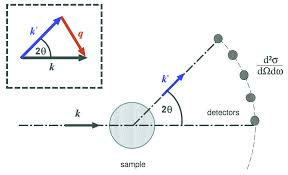
\includegraphics[width=5cm]{scat_CM.jpeg}
	\label{"halllo"}
\end{minipage}
\hfill
\begin{minipage}[hbt]{5cm}
	\centering
	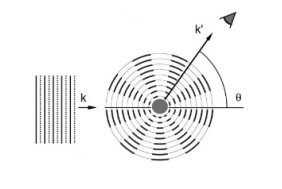
\includegraphics[width=5cm]{scat_QM.png}
	\label{Bild2}
\end{minipage}
\newline
\textit{Figure 2: Classical and quantum mechanical illustration of a neutron scattering off an atomic nucleus. 
To include thermodynamics, imagining the scattering centers to undergo a (correlated) random walk and take many overlain snapshots
of this random walk. Difference to text: $k$ labels $k_{in}$ and $k'$labels $k_{out}$.
If the incoming neutrons are not monochromatic, you may define the differential cross section per incoming frequency bin
$d \omega$ at a fixed $\omega$. (For inelastic scattering $\omega$ is the altered energy of the scattered neutron.)\newline
Discrepancy in caption: Since $q = 2k sin \frac{1}{2} \theta$ for elastic scattering,
$\theta$ as in the right image, it is convenient to define the angle of observation as $2\theta$. (As in the left image).} 
\newline
\newline
It is interesting that for an ideal gas the 'flying around' of atoms cannot be seen. 
(The cross section is temperature independent in this case.)
\newpage



\section{Computational Considerations}
\subsection{The OZ equations as a fix point problem}
We recall the set of Ornstein Zernike equations
\begin{equation}
h = c + \rho c*h \quad g = e^{-\beta u} f(\Gamma, B) \quad \Gamma = h -c \quad g = h+1
\end{equation}
$f$ in principle is a arbitrary function here, depending also on the bridge function $B$, so generically
$f = e^{\Gamma + B}$ but for PY or HNC will be $e^{\Gamma}$ or $1+ \Gamma$.
To arrive at a fix point formulation, we define the tuple $x = (h,c)$ containing the two unknown functions and rewrite the above equations as
\begin{equation}
c = h - \rho c*h \quad h = e^{-\beta u} f(\Gamma, B) -1
\end{equation}
Using $x$ 
\begin{equation}
x := (c,h) =: (G_1(c,h), G_2(c,h)) = (G_1(x), G_2(x)) =: G(x)
\end{equation}
The parameters of this fix point equation are $\rho, \beta, f$ and $u$, i.e fluid density, temperature, closure relation and two-particle potential.
(Particle diameter for a hard sphere potential). So a solution $x^{*}$ is dependent on these parameters
\begin{equation}
x^{*} = x^{*}(\rho, \beta, u,f)
\end{equation}
To make equation (49) amenable to numerical procedures, $h,c$ are discretized on 1D grid\footnote{isotropic fluids only}
with $n$ sampling points such that $h,c \in \mathbf{R}^{n}, x \in \mathbf{R}^{2n}$ and

\begin{equation}
G: \mathbf{R}^{2n} \rightarrow \mathbf{R}^{2n} \quad x \rightarrow G(x)
\end{equation}

The way the fix point problem is tackled in \texttt{SASfit} is using FFT's to avoid convolution. FFTing the OZ equation:
\begin{equation}
\hat h = \hat c + \rho \hat c \hat h \Leftrightarrow
\hat h - \rho \hat c \hat h = \hat c \Leftrightarrow
\hat h = \frac{\hat c}{1 - \rho \hat c}
\end{equation}
Plugging this into the definition of $\hat \Gamma$
\begin{equation}
\hat \Gamma = \hat h - \hat c =
\frac{\hat c}{1 - \rho \hat c} - \hat c =
\frac{\rho \hat c^{2}}{1 - \rho \hat c}
\, \Leftrightarrow \,
\Gamma =  \mathcal{F}^{-1} 
\Bigl\{
\frac{\rho \hat c^{2}}{1 - \rho \hat c}
\Bigr\}
\end{equation}

So far we only have used the OZ equation, hence now we use the closure relation for the direct correlation function
(Subtract $\Gamma$ from the second equation in (48) and FFT to get the closure, finally plug (54) into (53) to get a fix point problem
for $\Gamma$. Staying in Fourier space only works for PY).
\begin{equation}
\hat c = \mathcal{F} \bigl\{     e^{-\beta u} f(\Gamma, B)      \bigr\}
- \mathcal{F}(\Gamma) - \delta
\end{equation}


\subsection{Algorithms to solve the fix point problem}
All presented algorithms are iterative. Consider Markov noise numerical.
\subsubsection{Markov like algorithms}
With 'Markov like' we mean algorithms that only use the current state to infer the result of the next iteration. The simplest possible
algorithm to find the fixpoint of (51) is the Picard iteration
\begin{equation}
x_{k+1} = G(x_k)
\end{equation}
$G$ needs to be a contraction for this algorithm to work
\begin{equation}
\exists \lambda \in [0,1): \quad |G(x) - G(y)| \le \lambda|x -y| \quad \forall x,y \in \mathbf{R}^{2n}
\end{equation}

This way it is guaranteed that the error $e$, say at iteration 3, is smaller than at iteration 2:
\begin{equation}
e_3 := |x_3 - x_2| =|G(x_2) - G(x_1)| \le  \lambda|x_2 - x_1| < |x_2 - x_1| =:e_2
\end{equation}
the above chain obviously holds for all $k$ , such that the error is continuously decreasing ($\lambda < 1$), forcing the algorithm to
converge, though it may take very long. (The OZ fix point operator \textit{is} a contraction\footnote{Conversation with Joachim},
so Picard should always work). 
\newline
A more advanced iteration scheme is the (quasi) Newton method
\begin{equation}
x_{k+1} = x_k + (1 - G'(x_k))^{-1}(G(x_k) - x_k)
\end{equation}
A sufficient condition for the algorithm to be in state 'converged' is indeed $G(x_k) - x_k = 0$. To understand the specific formula,
we give a self-consistency argument. Say the algorithm is one step before being converged, $x_{k+1} = x^{*}$, $\Delta x_k = x^{*} - x_k$
and $G(x^{*}) = x^{*}$

\begin{equation}
\Delta x_k = x^{*} - x_k = (1 - G'(x_k))^{-1}(G(x^{*} - \Delta x_k) - (x^{*} - \Delta x_k))
\end{equation}

Now $G(x^{*} - \Delta x_k)$ is first order expanded as 
\begin{equation}
G(x^{*} - \Delta x_k) \simeq G(x^{*}) - G'(x^{*})\Delta x_k = x^{*} - G'(x^{*})\Delta x_k
\end{equation}


Inserting this into the above equation
\begin{equation}
\Delta x_k = x^{*} - x_k = (1 - G'(x_k))^{-1}(x^{*} - G'(x^{*})\Delta x_k - x^{*} + \Delta x_k)
\end{equation}

or
\begin{equation}
\Delta x_k = (1 - G'(x_k))^{-1} (1 - G'(x^{*}))\Delta x_k
\end{equation}

This shows that the mathematics is correct near the fix point. (The formula also shows that it would be better to take $G'(x_{k+1})$ in (58),
but this is not available). \newline
The problem with Newton algorithms is that in every step one has to calculate first the Jacobi Matrix and then perform a
Matrix inversion, this is expensive and may be numerically unstable. (Recall that $G'$ is a matrix with millions of entries for OZ).
The advantage is that $G$ needs not be a contraction. (Which is however irrelevant for OZ).

\subsubsection{Non Markov like algorithms}
With non-Markov like algorithms we mean that additional past states are involved in the calculation of the current state.
Many different flavours are available in \texttt{SASfit}, a simple form is e.g the Krasnoselskij iteration
\begin{equation}
x_{k+1} = (1 - \alpha) x_k + \alpha G(x_k) \quad
\alpha \in (0,1]
\end{equation}

The Mann iteration is structurally the same, but now $\alpha$ is altered dynamically
\begin{equation}
x_{k+1} = (1 - \alpha_k) x_k + \alpha_k G(x_k) \quad
\alpha_k \in (0,1]
\end{equation}

There are many more, one of the most performant seems to be the Anderson Acceleration method. Here a number of past states $m$
is used to calculate the new state as follows: At step $k > m$ a Matrix $X_k$ was built up to contain the past $m$ states $x_{k-j}$, $\, j=0...m-1$
and a Matrix $R_k$ was built up to store the past $m$ residuals $r_{k-j}$, $\, j=0...m-1$ where $r_k = x_k - x_{k-1}$. 
The mixing coefficients $\alpha \in \mathbf{R}^{m}$ are now defined to minimize $|| R_k \alpha ||$

\begin{equation}
\alpha_{k+1} = \min_{\alpha} || R_k \alpha || \quad s.t. \sum_i \alpha_i = 1
\end{equation}
The idea is that if the coefficients $\alpha$ are good at making the last residuals small, they are as well suited to find
the new state
\begin{equation}
x_{k+1} = X_k \alpha_{k+1} = \sum_j \alpha_{k+1}[j]x_j
\end{equation}

where $x_j$ are the columns of $X_k$ (the previous states). \newline This justification is a bit vague (making the residuals smaller
is fine, but why should the same coefficients also allow for a good new state? I did not fully understand why AAA is so
powerful for this problem.)\newline
The Non-Markov property is most apparent for AAA. For Mann or Krasnoselskij the notion of a 'previous' state may be a bit confusing.
Comparing with Picard, where $x_{k+1} = G(x_k)$ one can at least see that mixing  $x_{k}$ and $G(x_k)$ combines two different iteration
stages, irrespective of whether they are called 'past' or 'future'. And, in this sense, the Newton algorithm described in the previous
chapter is also Non-Markovian.
\newpage


\section{Appendix}
\subsection{Analytical solution for the 3-particle bridge function}
The idea of the bridge function $B$ is to find the radial distribution function $g$. Conversely, if we knew $g$, we could infer $B$

\begin{equation}
e^{B} = g e^{\beta U} e^{-\Gamma}
\end{equation}

We write the FFT of $\Gamma$ as
\begin{equation}
\hat \Gamma = \frac{\rho \hat h^2}{1 + \rho \hat h}
=
\frac{\rho (\hat g - \delta)^2}{1 + \rho (\hat g - \delta)}
\end{equation}
Since the square of a $\delta$ distribution is mathematically not well-defined, we go back to real space
\begin{equation}
\Gamma =
\rho (g - 1)*(g - 1)*
\mathcal{F}^{-1}\frac{1}{1 + \rho (\hat g - \delta)}
\end{equation}

Since for convolution its holds distributivity (and associativity plus commutativity) there is
\begin{equation}
(g - 1)*(g - 1) = g*g - 2g*1 + 1*1 =
g*g - k_1
\end{equation}
where the constant $k_1$ equals $2 \int g d \vec r + V$. Hence
\begin{equation}
\Gamma =
\rho (g*g - k_1)*
\mathcal{F}^{-1}\frac{1}{1 + \rho (\hat g - \delta)}
\end{equation}


Using the explicit result (25) for the 3 particle pair distribution and defining the pair potential Boltzmann factor 
$e^{-\beta u}$ as $b$
\begin{equation}
g = k_2 b(b*b)
\end{equation}

Hence (67) becomes
\begin{equation}
e^{B} = k_2 (b*b) e^{-\Gamma} \, \Leftrightarrow \,
B = \ln (k_2) + \ln(b*b) - \Gamma
\end{equation}
Using (71) for $\Gamma$ and inserting the result for $g$

\begin{equation}
B = \ln (k_2) + \ln(b*b) - \rho \{ k_2^2 [b(b*b)]*[b(b*b)] - k_1 \}*
\mathcal{F}^{-1} \Big\{
\frac{1}{1 + \rho [k_2 \mathcal{F}\{ b(b*b) \} - \delta]}
\Big\}
\end{equation}

This is admittedly not nice, but nevertheless an analytical expression of $B$ in terms of $b$. (In functional language,
there is $B = B[b]$ or $B = B[e^{-\beta u}]$). The result holds for any pairwise additive parity symmetric potential.

\newpage
\subsection{Form Factors}
In order to derive eq. (45), it was necessary to assume a sum of delta-potentials seen by the scattered neutrons on their
way through the liquid. A more involved potential $V$ can be written as $V*\delta$, this gives the connection to
the derived cross section above. \footnote{This is similar to Coulomb scattering, where the Potential of a point source is $V_{ps} \propto \frac{1}{r}$
and the potential of a charge cloud $\rho$ equals $V = \frac{1}{r} * \rho $
and hence $\frac{d \sigma} {d\Omega} \propto |\hat V|^2 = (\frac{d \sigma} {d\Omega})_{ps} |\hat \rho|^2$}
\begin{equation}
V(\vec r) = \sum_i V(\vec r - \vec r_i) = 
\sum_i V(\vec r) * \delta(\vec r - \vec r_i) =
V (\vec r) * \sum_i \delta(\vec r - \vec r_i)
\end{equation}

where the sum runs over all particle positions (the center of mass of the atoms or molecules).
So we write $V_{neutron-nuclei} = V*V_{ps}$, i.e. the total potential equals the convolution of the atomic/molecular potential and the
point-source potential of the particle locations. The transition probability is modified according

\begin{equation}
|\mathcal{F} (V) (\vec q)|^2 =
|\mathcal{F} (V*V_{ps}) (\vec q)|^2 =
|\mathcal{F} (V) \mathcal{F}(V_{ps}) (\vec q)|^2 =
|\mathcal{F} (V)(\vec q)|^2 |\mathcal{F}(V_{ps}) (\vec q)|^2
\end{equation}
where the convolution theorem was applied. To calculate the thermal average, we first assume a potential $V$ which is not affected 
by the the heat bath induced thermal fluctuations, this is e.g the case for a mono-atomic liquid with a complex nucleus. 
(Say the nucleus cannot be thermally excited and is too large to be approximated by a delta potential).
\begin{equation}
\langle |\hat V (\vec q)|^2  | \hat V_{ps}(\vec q)|^2 \rangle
= |\hat V (\vec q)|^2 \langle   | \hat V_{ps}(\vec q)|^2 \rangle
\end{equation}
For a molecule the situation is more complicated, since the nuclei within the molecule are definitely affected by thermal
fluctuations. But if we postulate that the intra-molecular thermal fluctuations are independent of the inter-molecular fluctuations,
i.e. the random  walk of the molecule as a whole is neither correlated to the random jiggling of its constituent nor to the rotation of the molecule,
\footnote{This is not true on a microscopic scale, but may hold on average} we can write
\begin{equation}
\langle |\hat V (\vec q)|^2  | \hat V_{ps}(\vec q)|^2 \rangle
= \langle|\hat V (\vec q)|^2 \rangle \langle   | \hat V_{ps}(\vec q)|^2 \rangle
\end{equation}
and hence express the differential cross section  as
\begin{equation}
\langle \frac{d \sigma} {d\Omega} \rangle = 
\langle \frac{d \sigma} {d\Omega} \rangle_{ps}
\langle|\hat V (\vec q)|^2 \rangle
=
\frac{m^2}{4 \pi^2 \hbar^4} N
\langle|\hat V (\vec q)|^2 \rangle (1 + \rho \hat g)
\end{equation}

where here $\langle | \hat V (\vec q)|^2 \rangle$ is the thermal expectation value of the cross section of a single molecule.
\newpage
For a contact-interaction like the neutron-nucleus interaction, there is $V \propto \rho_N$, where $\rho_N$ denotes
the nuclei-distribution within the molecule. (Compare to equation (75)). Equation (79) takes the more familiar form
\begin{equation}
\langle \frac{d \sigma} {d\Omega} \rangle 
\propto
\langle \frac{d \sigma} {d\Omega} \rangle_{ps}
\langle|\hat \rho_N|^2 \rangle
\propto
\langle|\hat \rho_N|^2 \rangle N (1 + \rho \hat g)
\end{equation}

The proportionality between $V$ and $\rho_N$ holds for a single-type molecular liquid and the molecule itself
must have equal nuclei (including spin and isotope, see e.g. pure spin zero $^{16}$O$_2$), then $b\rho \propto V$, $b$ being the scattering length.
\newline
Remark regarding units: Often the single nucleon Fermi pseudo potential is defined as 
\begin{equation}
V(\vec r) = \frac{2 \pi \hbar^2}{m} b \delta(\vec r)
\end{equation}
The convenient property of this definition is that the factor  $|\frac{2 \pi \hbar^2}{m}|^2$ cancels with the factor 
$\frac{m^2}{4 \pi^2 \hbar^4}$ derived in the cross section formula. 
\footnote{And indeed the scattering length $b$ has then length units. (Remember that $\delta$ has inverse Volume units).}
However, for this definition, the factor reappears in the proportionality between $V$ and $\rho_N$.
\newline
To be specific, we examine the simplest possible generalization to the mono atom liquid, the homonuclear diatomic liquid 
(e.g. $H_2$). We refer to [\cite{sears}] in the following. The neutron-liquid interaction for a homonuclear diatomic liquid can be written as


\begin{equation}
V(\vec r, \vec S) = \frac{2 \pi \hbar^2}{ m}
\sum_{j} \sum_{\gamma = \pm 1} (b_c + b_i \vec S \vec I_{j \gamma}) \delta(\vec R_j + \frac{1}{2} \gamma \vec r_j - \vec r)
\end{equation}

where $\vec r, \vec S$ is the position, spin of the neutron respectively, $\vec R_j$ is the center of mass position of molecule $j$, $\vec r_j$
the intra-atomic distance between the two nuclei and $\vec I_{j \gamma}$ is the nuclear spin of atom $\gamma$ in molecule $j$. 
$b_c, b_i$ is the coherent, incoherent scattering length respectively. The inelastic differential cross section reads

\begin{equation}
\frac{d \sigma}{ d \Omega d \omega} =
\frac{k_{out}}{k_{in}}
\sum_{s' }\sum_{m,m'} \sum_{n,n'} P_{nm} | \langle \vec k_{out}, s'; n', m' | \tilde V | \vec k_{in}, s; n, m \rangle |^2
\delta \bigl\{ \omega + \frac{ E_{nm} - E_{n'm'} } {\hbar} \bigr\}
\end{equation}

where a free liquid state is assumed to be split into a free molecular part $m$ and a free nuclear part $n$. $\omega$
equals the energy transferred from the neutron to the liquid, $\hbar \omega = \hbar^2 /2m (k_{in}^2 - k_{out}^2)$. 
$s'$ is the final spin of the neutron, $s$ its incoming spin. \newline
To calculate the cross section, we calculate first the quantum mechanical expectation value of the spatial
part of the neutron which again is a Fourier transform ($ \int d \vec r e^{i\vec q \vec r}$) 


\begin{equation}
\langle \vec k_{out} | \tilde V | \vec k_{in} \rangle = 
\sum_{j} \sum_{\gamma = \pm 1} 
b_c e^{i \vec q \vec R_j} e^{i \vec q \frac{1}{2} \gamma \vec r_j} 
+
\sum_{\gamma = \pm 1} 
b_i \vec S \vec I_{j \gamma} e^{i \vec q \vec R_j} e^{i \vec q \frac{1}{2} \gamma \vec r_j} 
\end{equation}

evaluating the sum over atoms (and using Euler's formula and the parity (anti-) symmetry of the sine and cosine function)

\begin{equation}
\langle \vec k_{out} | \tilde V |\vec k_{in} \rangle = 
\sum_{j} a_j (\vec q) e^{i \vec q \vec R_j} 
\end{equation}

where
\begin{equation}
a_j(\vec q) = A_j \cos ( \vec q \vec r_j/2) + i B_j \sin (\vec q  \vec r_j/2)
\end{equation}

and 
\begin{equation}
A_j = 2 b_c + 2 b_i \vec S ( \vec I_{j, +} + \vec I_{j, -}) \quad
B_j = 2 b_i \vec S (\vec I_{j, +} - \vec I_{j, -} )
\end{equation}

Note that setting $b_i = 0$ and $\vec r_j = 0$ we get the same result as for the mono atomic liquid, except for the factor 2, since there are
two atoms sitting at the same place in this simplification. \newline 
As the next steep, we must evaluate the remaining average (both thermal and quantum mechanical)

\begin{equation}
\frac{d \sigma}{ d \Omega d \omega} =
\frac{k_{out}}{k_{in}}
\sum_{s' }\sum_{m,m'} \sum_{n,n'} P_{nm} | \langle s'; n', m' | \sum_{j} a_j (\vec q) e^{i \vec q \vec R_j}  | s; n, m \rangle |^2
\delta \bigl\{ \omega + \frac{ E_{nm} - E_{n'm'} } {\hbar} \bigr\}
\end{equation}

To do so, we rewrite the quantum mechanical transition probability as
\begin{equation}
\begin{split}
| \langle s'; n', m' | \sum_{j} a_j (\vec q) e^{i \vec q \vec R_j}  | s; n, m \rangle |^2  \\
=
\langle s; n, m  | \sum_{j} a_j^{*} (\vec q) e^{-i \vec q \vec R_j}  | s'; n', m' \rangle 
\langle s'; n', m' | \sum_{j} a_j (\vec q) e^{i \vec q \vec R_j}  | s; n, m \rangle 
\end{split}
\end{equation}

where $a_j^{*}$ denotes the Hermitian conjugate operator. (The molecular position operator $\vec R_j$ is self-adjoint).
Since we sum over all final states $s',n',m'$, and since these states form a basis in the considered part of the Hilbert space,
we could make use of the fact that $\sum_{s', n',m' }| s', n', m'  \rangle \langle s', n' , m' |= 1$, but the
delta function opposes this plan. To get rid of the delta, we rewrite it as
\begin{equation}
\delta \bigl\{ \omega + \frac{ E_{nm} - E_{n'm'} } {\hbar} \bigr\} =
\int e^{- i \omega t} e^{- iE_{nm} t / \hbar} e^{i E_{n'm'}t / \hbar} dt
\end{equation}
and use the fact that $e^{iE_{n'm'} t / \hbar} |n',m' \rangle = U^*(t) |n',m' \rangle$, where $U(t) $ is the evolution operator of the free 
system described by the Hamiltonian $H_0$, $U(t) = e^{- i H_0 t / \hbar}$.
The other factor $e^{-iE_{nm} t / \hbar}$ is absorbed as $U(t) |m, n \rangle $ such that

\begin{equation}
\frac{d \sigma}{ d \Omega d \omega} =
\frac{k_{out}}{k_{in}}
\int d t e^{-i\omega t}
\sum_{nm}  P_{nm} 
\langle s; m, n | 
\sum_{j'} a_{j'}^{*} (\vec q) e^{-i \vec q \vec R_{j'}} 
\sum_{j} U^*(t) a_j (\vec q) e^{i \vec q \vec R_j}   
 U (t) | s; m, n \rangle
\end{equation}

The next simplification is to assume that the evolution operator factorizes in a product according molecular and nuclear
time evolution: $U(t) = U_n(t) \otimes U_m(t)$. \footnote{This implies that the full Hamiltonian $H_0$ is a sum of molecular
and nuclear Hamiltonian $H_0= H_{0, n} + H_{0, m}$ and alike for the energy $E_{nm}= E_n + E_m$}
As already mentioned, this is not strictly true, since the molecular collisions could induce intra-molecular transitions.

\begin{equation}
\frac{d \sigma}{ d \Omega d \omega} =
\frac{k_{out}}{k_{in}}
\mathcal{F}_t
\sum_{nm}  P_{nm}
\langle s; m, n | 
\sum_{j'} a_{j'}^{*}(\vec q) e^{-i \vec q \vec R_{j'}} 
\sum_{j} U_n^*(t)a_j(\vec q) U_n(t) U_m^*(t)e^{i \vec q \vec R_j}  U_m (t)  
| s; m, n \rangle
\end{equation}

Writing the time evolved operators according the Heisenberg picture notion
\begin{equation}
\frac{d \sigma}{ d \Omega d \omega} =
\frac{k_{out}}{k_{in}}
\mathcal{F}_t
\sum_{nm}  P_{nm} 
\langle s; m, n | 
\sum_{j'} a_{j'}^{*} (\vec q) e^{-i \vec q \vec R_{j'}} 
\sum_{j}a_j (\vec q, t) e^{i \vec q \vec R_j(t)}   
| s; m, n \rangle
\end{equation}

This equals
\begin{equation}
\frac{d \sigma}{ d \Omega d \omega} =
\frac{k_{out}}{k_{in}}
\mathcal{F}_t
\sum_{nm}  P_{nm} 
\sum_{jj'} 
\langle s, n| 
a_{j'}^{*} (\vec q) a _j (\vec q, t) | s, n \rangle
\langle m| e^{-i \vec q \vec R_{j'}} 
e^{i \vec q \vec R_j (t)}   
| m \rangle
\end{equation}


Since $P_{nm} = e^{-\beta (E_n + E_m)}/(Z_n Z_m) = P_n P_m$ we rewrite this as
\begin{equation}
\frac{d \sigma}{ d \Omega d \omega} =
\frac{k_{out}}{k_{in}}
\mathcal{F}_t
\sum_{jj'}
\sum_{n}  P_{n} \langle s, n| 
a_{j'}^{*} (\vec q) a_j (\vec q, t) | s, n \rangle
\sum_{m}  P_{m} 
\langle m| e^{-i \vec q \vec R_{j'}} 
e^{i \vec q \vec R_j (t)}   
| m \rangle
\end{equation}

This can be written as
\begin{equation}
\frac{d \sigma}{ d \Omega d \omega} =
\frac{k_{out}}{k_{in}}
\mathcal{F}_t
\sum_{jj'}
\langle a_{j'}^{*} (\vec q) a_j (\vec q, t) \rangle_{T_n}
\langle e^{-i \vec q \vec R_{j'}} e^{i \vec q \vec R_j (t)} \rangle_{T_m}
\end{equation}

where the subscript $T$ was added to specify the thermal average is taken of the operators $a_{j'}^{*} (\vec q) a_j (\vec q, t)$
and $e^{-i \vec q \vec R_{j'} } e^{i \vec q \vec R_j(t)}$


Note that for $a_j (\vec q) =1$ it holds $a_{j'}^{*} (\vec q, t) = 1$ and the cross section coincidences with the mono atomic liquid.
($\sum_n P_n = 1$ and $\langle s,n | s, n \rangle = 1$). As for the mono atomic liquid, the sum is split into $j = j'$ and $j \ne j$.
For different molecules in a homogeneous liquid, we again assume that the contribution is identical for all pairs
$j \ne j'$. To evaluate the nuclear part contribution of say molecule 1 and 2, we write a total nuclear state
$|n \rangle $ explicitly as the product over all molecules $|n \rangle = |n_1 \rangle |n_2 \rangle ...  |n_N \rangle $, where
$|n_1 \rangle$ is the state describing the molecular part of molecule 1 etc. The total internal energy is accordingly $E_1 + ... + E_N$
and the Boltzmann probabilities factorize as well $P_n = P_{n_1}....P_{n_N}$ where all single molecule internal probabilities are
normalized: $\sum_l P_{n_i, l} = 1$, where $P_{n_i, l}$ is the probability to find a molecule $i$ in internal state $l$.
With these prerequisites, we can calculate 

\begin{equation}
\langle a_{1}^{*} (\vec q) a_2 (\vec q, t) \rangle_T =
\sum_l P_{n_1, l}  \langle l | a_{1}^{*}|l \rangle
\sum_{l'} P_{n_2, l'}  \langle  l' | a_2 (\vec q, t) |l' \rangle
\end{equation}

Since again for a homogeneous system nothing discriminates molecule 1 from molecule 2, there is

\begin{equation}
\langle a_{j}^{*} (\vec q) a_{j'} (\vec q, t) \rangle_{T_{n_j;n_{j'} } }=
\langle a_{1}^{*} (\vec q)  \rangle_{T_{n_1}}
\langle a_{2} (\vec q, t) \rangle_{T_{n_2}}
=
\langle a_{1}^{*} (\vec q)  \rangle_{T_{n_1}} \langle a_{1} (\vec q, t) \rangle_{T_{n_1}}
\end{equation}


where on the right hand side the thermal average is taken for one single molecule (labeled 1, the equation simply
states that molecule $j$ and $j'$ are decorrelated for all times if $j \ne j'$). \newline
For the sum with equal $j$ terms, we chose as well the first molecule as representative for the identical
thermal averages

\begin{equation}
\langle a_{j}^{*} (\vec q) a_{j} (\vec q, t) \rangle_T =
\sum_l P_{n_1, l}  \langle l | a_{1}^{*} (\vec q) a_1 (\vec q, t) |l \rangle =
\langle a_{1}^{*} (\vec q) a_1 (\vec q, t)\rangle_{T_{n_1}}
\end{equation}

This finally allows us to write the differential cross section as (omitting thermal subscript)

\begin{equation}
\begin{split}
\frac{d \sigma}{ d \Omega d \omega} =
\frac{k_{out}}{k_{in}}
\mathcal{F}_t
\biggl\{
\langle a_{1}^{*} (\vec q) a_1 (\vec q, t)\rangle
\sum_{j} \langle e^{-i \vec q \vec R_{j}} e^{i \vec q \vec R_j (t)} \rangle
\, +
\\
\langle a_{1}^{*} (\vec q)  \rangle \langle a_{1} (\vec q, t) \rangle
\sum_{j \ne j' }\langle e^{-i \vec q \vec R_{j'}} e^{i \vec q \vec R_j (t)} \rangle
\biggr\}
\end{split}
\end{equation}


Since the two different sums are differently weighted according the nuclear form factor, one cannot split the cross section
in a product (or convolution) of the form 'form factor times point cross section'. \newline
The rest of this section is devoted to calculate the form factor. The so far summarized internal degrees of freedom $|n \rangle$
of the molecule are a set of quantum numbers: $n$ describing the relative radial motion of the intra-molecular nuclei, 
quantum numbers $l, m$ describing the rotation of the nuclei around the common center of mass and quantum numbers $T, m_T$ describing
the total spin of the two coupled nuclear spins. Hence a internal nuclear state is of the form $|\psi_n(r) Y_{lm} (\theta, \phi) \rangle
\otimes | T, m_T \rangle$. In the following, it is assumed that the two nuclei are fermions, hence the total nuclear wave function
needs to be antisymmetric. $\psi_n(r)$ is symmetric for all $n$, whereas the spherical harmonics 
$Y_{lm}$ transforms under parity ($\vec r := \vec r_1 - \vec r_2 \rightarrow \vec r_2 - \vec r_1 = -\vec r$) as 
$Y_{lm}(\pi - \theta, \pi + \phi) = (-1)^l Y_{lm} (\theta, \phi)$. So for odd $l$, the spatial wave function changes sign under parity and
consequently the spin 'wave function' should not change sign, i.e. be symmetric to keep the overall wave function antisymmetric.
So we turn to the total nuclear spin $\vec T = \vec I_{+} + \vec I_{-}$. The $SU(2)$ representation of the total spin is

\begin{equation}
D^{I} \otimes D^{I} = D^{2I} \oplus \ D^{2I -1 } \oplus \cdots \oplus D^1 \oplus D^0 = \sum_{T = 0}^{2I} D^{T}
\end{equation}

The right hand side sum corresponds to eigenstates $|T \rangle$ of total nuclear spin. Now an evenly represented total spin
is antisymmetric whereas a oddly represented spin is symmetric under particle exchange. (E.g $I = 1/2$, singlet $T=0$ is antisymmetric
and triplet $T=1$ is symmetric). Hence for fermions, the following rule applies: Even total nuclear spin $T$ goes with even angular momentum $l$,
odd total nuclear spin $T$ goes with odd angular momentum $l$. Otherwise stated: $|l,m  \rangle | T, m_T \rangle$ is valid state (can be occupied) for $l + T$ even.
\footnote{This restriction would not be present for Boltzmann particles and is 'inverted' for bosons.}
Doing Boltzmann statistics, this leads to the next questions. How many (anti-)symmetric spins states are there?

\begin{equation}
N_{I,sym} = \sum_{T odd}^{2I} 2T + 1 = (2I + 1)I    \quad
N_{I,asym} = \sum_{T even }^{2I}  2T + 1 =  (2I + 1)(I + 1)
\end{equation}

As a sanity check, we calculate the total number of nuclear spin states

\begin{equation}
N_{I} = N_{I,sym} + N_{I,asym}
= (2I + 1)I + (2I + 1)(I + 1)
= (2I + 1)^2
\end{equation}

as it should be. \newline
Knowing the statistics of the nuclear states, we are prepared to calculate the form factors of eq (100). The different-molecule form factor
can be simplified due to $\langle a(\vec q, t) \rangle = \langle a(\vec q) \rangle$ and $\langle a^*(\vec q) \rangle = \langle a(\vec q) \rangle ^*$
where the second asterisk denotes complex conjugation. 
\footnote{Boltzmann factors are real and $\langle x, A^* x \rangle = \langle A^* x ,x \rangle^* = \langle x , A x \rangle^*$}
Hence

\begin{equation}
\langle a_{1}^{*} (\vec q)  \rangle \langle a_{1} (\vec q, t) \rangle
=
| \langle a_{1} (\vec q) \rangle |^2
=
| \sum_{\alpha }  P_{\alpha} \langle \alpha | a_{1} (\vec q) | \alpha \rangle |^2
\end{equation}

For the identical-molecule term  we cannot get rid of the time dependence, since $[U_i, a_i] \ne 0$, hence we must revert the program which lead to eq. (100)
to some extend and reintroduce a complete set of (energy eigen-) states $|\beta \rangle = |s, m \rangle$.


\begin{equation}
\langle a_{1}^{*} (\vec q) a_1 (\vec q, t)\rangle
=
\sum_{\alpha \beta} P_{\alpha} 
\langle \alpha | a_{1}^{*} (\vec q)|\beta \rangle \langle \beta | U^* a_1 (\vec q) U |  \alpha \rangle
\end{equation}

using the fact that $\alpha$ and $\beta$ are energy eigenstates

\begin{equation}
\langle a_{1}^{*} (\vec q) a_1 (\vec q, t)\rangle
=
\sum_{\alpha \beta} P_{\alpha} e^{-i E_{\alpha}t/\hbar } e^{i E_{\beta} t/\hbar}
\langle \alpha | a_{1}^{*} (\vec q)|\beta \rangle \langle \beta | a_1 (\vec q) |  \alpha \rangle
\end{equation}

and hence \footnote{$\langle x, A^* y \rangle = \langle A^* y ,x \rangle^* = \langle y , A x \rangle^*$}

\begin{equation}
\langle a_{1}^{*} (\vec q) a_1 (\vec q, t)\rangle
=
\sum_{\alpha \beta} P_{\alpha} e^{-i E_{\alpha}t/\hbar } e^{i E_{\beta} t/\hbar}
| \langle \beta | a_1 (\vec q) |  \alpha \rangle |^2
\end{equation}
So we are left with calculating all the matrix elements of the operator $a_1 (\vec q)$. (The 1 subscript is dropped, since
any molecule may be chosen.). We chose form (106) which is more convenient
\begin{equation}
\langle \beta | a (\vec q) |  \alpha \rangle
=
\langle m_s', n', l',m', T', m_T' | a (\vec q) | m_s,n, l,m,T,m_T \rangle
\end{equation}
\begin{equation}
\langle \alpha | a^* (\vec q) |  \beta \rangle
=
\langle m_s, n, l,m, T, m_T | a^* (\vec q) | m_s',n', l',m',T',m_T' \rangle
\end{equation}

If the liquid is cold enough the molecular oscillatory degrees of freedom are not thermally excited and if in turn the scattered neutrons
are cold enough the oscillatory states won't be excited by a scattering event, hence we can assume that $n = n' =0$ and drop this index
\footnote{The Boltzmann factors of these states are tiny. The oscillator ground state is typically as Gaussian} \newline
In order to calculate the sum in equation (107), we exploit the fact that the energy (and hence both the Boltzmann factors
$P_{\alpha}$ and the time oscillations  $e^{-i E_{\alpha}t/\hbar }$) only depend on the quantum number $l$, hence we
again use the fact that the quantum numbers forming state $\beta$ but $\ne l$ form a basis in their subspace, i.e
$\sum_{m_s',T',m_T'} |m_s',T',m_T' \rangle \langle m_s', T',m_T'| = 1 $ such that \footnote{This would not be possible if the free Hamiltonian
contained a nuclear spin-spin interaction term $\propto \vec I_{+}\vec I_{-}$.}
\begin{equation}
\langle a^{*} (\vec q) a (\vec q, t)\rangle
=
\sum_{ \alpha} P_{\alpha} e^{-i E_{\alpha}t/\hbar } e^{i E_{\beta} t/\hbar}
\langle \alpha | a_{1}^{*} (\vec q)|\beta \ne spin \rangle \langle \beta \ne spin| a_1 (\vec q) |  \alpha \rangle
\end{equation}

\newpage
The first 'matrix element' reads (it is actually an operator)
\begin{equation}
\langle l,m | \cos (\vec q \vec r /2)|  l',m' \rangle \langle m_s, T, m_T | A^*
- i
\langle l,m | \sin (\vec q \vec r /2)|  l',m' \rangle \langle m_s, T, m_T | B^*
\end{equation}

The second matrix element reads

\begin{equation}
 A |m_s, T, m_T \rangle \langle l',m' | \cos (\vec q \vec r /2)|  l,m \rangle
+ i
 B |m_s, T, m_T \rangle \langle l',m' | \sin (\vec q \vec r /2)|  l,m \rangle
\end{equation}



The matrix elements of the sine and cosine operator are
\begin{equation}
\langle l',m' | \cos (\vec q \vec r /2)|  l,m \rangle
=
\int  
|\psi_{0}(r)|^2 Y_{l'm'}^*(\theta, \phi) \cos (\vec q \vec r /2)   Y_{lm}(\theta, \phi) 
d \vec r
\end{equation}

and accordingly for the sine function. These functions correspond to the sine/cosine transformation of the function
$f_{l'm'lm}(\vec r) = |\psi_{0}|^2 Y_{l'm'}^* Y_{lm}$ and we label them as
$\hat f_{l'm'lm}^c (\vec q /2)$ and $\hat f_{l'm'lm}^s (\vec q /2)$ \newline
When we now combine operators (111) and (112), the cross products vanish, since a) Operator A and B are self adjoint,
($b_c$ and $b_i$ must be real numbers) b) $[A,B] = 0$ (all operators making up $A$ and $B$ live in different spaces) and c) 
since the energy is not $m$ dependent,one can calculate the sum over $m, m'$ for fixed $l,l'$ of the functions $e^{im \phi}$,
this sum is real such that e.g. $\sum_{m,m'}\langle l',m' | \cos (\vec q \vec r /2)|  l,m \rangle$ is real.


Hence the product of the matrix elements under investigation equals
\begin{equation}
\begin{split}
\langle \alpha | a_{1}^{*} (\vec q)|\beta \rangle \langle \beta | a_1 (\vec q) |  \alpha \rangle =
|\hat f_{l'm'lm}^c (\vec q /2)|^2 \langle m_s, T, m_T | A^* A |m_s, T, m_T \rangle \\ +
|\hat f_{l'm'lm}^s (\vec q /2)|^2 \langle m_s, T, m_T | B^* B |m_s, T, m_T \rangle 
\end{split}
\end{equation}

such that the equal molecule (or incoherent) form factor can be written
\begin{equation}
\begin{split}
\frac{1}{Z_n} \sum_{l,l'} e^{-\beta E_l} e^{i (E_{l'} - E_{l})  t /\hbar }
\sum_{m = -l,m'=-l'}^{l,l'} |\hat f_{l'm'lm}^c (\vec q /2)|^2
\sum_{T = 0, m_T = -T}^{2I, T} || A |m_s, T, m_T \rangle ||^2 \\ +
\frac{1}{Z_n} \sum_{l,l'} e^{-\beta E_l} e^{i  (E_{l'} - E_{l}) t /\hbar }
\sum_{m = -l,m'=-l'}^{l,l'} |\hat f_{l'm'lm}^s (\vec q /2)|^2
\sum_{T = 0, m_T = -T}^{2I, T} ||B |m_s, T, m_T \rangle ||^ 2
\end{split}
\end{equation}

where in both terms $l + T$ is even. 

%Since $|\hat f_{l'm'lm}^{c,s} (\vec q /2)|^2$ equals
%\begin{equation}
%\int  |\psi_{0}(r)|^4 
%Y_{l'm'}^*(\theta, \phi) (c,s) (\vec q \vec r /2)   Y_{lm}(\theta, \phi) 
%Y_{l'm'}(\theta', \phi') (c,s) (\vec q \vec r' /2)  Y_{lm}^*(\theta', \phi')
%d \vec r d \vec r'
%\end{equation}

The canonical partition function for the intra molecular system being

\begin{equation}
Z_n = N_{I,asym} \sum_{l \,even} (2l + 1) e^{-\beta E_l} +  N_{I,sym} \sum_{l \,odd} (2l + 1) e^{-\beta E_l} 
\end{equation}

and the rotational energy (in rigid rotor approximation)

\begin{equation}
E_l = l(l+1)\hbar^2/(2I_m)
\end{equation}

where $I_m$ is the molecular moment of inertia. \newline For Boltzmann particles, where the exclusion principle induced
spin-orbit coupling is missing, the incoherent form factor simplifies as


\begin{equation}
\begin{split}
\frac{Tr(A^*A)}{\tilde Z_n} \sum_{l,l'} e^{-\beta E_l} e^{i (E_{l'} - E_{l})  t /\hbar }
\sum_{m,m'} |\hat f_{l'm'lm}^c (\vec q /2)|^2
\\ + \,
\frac{Tr(B^*B)}{\tilde Z_n} \sum_{l,l'} e^{-\beta E_l} e^{i  (E_{l'} - E_{l}) t /\hbar }
\sum_{m, m'} |\hat f_{l'm'lm}^s (\vec q /2)|^2
\end{split}
\end{equation}

where
\begin{equation}
\tilde Z_n = N_{I} \sum_{l} (2l + 1) e^{-\beta E_l} \quad
=: Z_{spin} Z_l
\end{equation}

The coherent form factor equals (originating from different Boltzmann particles)

\begin{equation}
\biggr\rvert
\frac{ Tr(A)} {\tilde Z_n} \sum_{l} e^{-\beta E_l} \sum_{m} \hat f_{lmlm}^c (\vec q /2) 
+  i
\frac{ Tr(B)}{\tilde Z_n} \sum_{l} e^{-\beta E_l} \sum_{m} \hat f_{lmlm}^s (\vec q /2)
\biggl\lvert ^2
\end{equation}
Recalling the definition of $f_{lmlm}^c$, $f_{lmlm}^s$  and using the fact that $\sum_m |Y_{lm}|^2 = \frac{2l +1}{4 \pi}$
(Additionstheorem)

\begin{equation}
\begin{split}
\frac{1}{16 \pi^ 2}
\biggr\rvert
\frac{ Tr(A) }{Z_{spin}} \hat g^c (\vec q /2) \sum_{l} (2l +1)e^{-\beta E_l} /Z_l
\\ + \, i
\frac{ Tr(B) }{Z_{spin}} \hat g^s (\vec q /2) \sum_{l} (2l +1)e^{-\beta E_l} /Z_l
\biggl\lvert ^2
\end{split}
\end{equation}

where 
\begin{equation}
\hat g^c =
\int  
|\psi_{0}(r)|^2  \cos (\vec q \vec r /2)
d \vec r
=
Re \mathcal{F} (|\psi_{0}|^2)(\vec q \vec r /2)
\end{equation}
\begin{equation}
\hat g^s =
\int  
|\psi_{0}(r)|^2  \sin (\vec q \vec r /2)
d \vec r
=
Im \mathcal{F} (|\psi_{0}|^2)(\vec q \vec r /2)
\end{equation}

Since $\hat g^s = 0$ this equals
\begin{equation}
\frac{1}{16 \pi^ 2}
\frac{Tr^2(A) }{Z_{spin}^2 }
|\hat g (q /2)  | ^2    \quad 
\hat g = \mathcal{F} (|\psi_{0}|^2)
\end{equation}
which reminds the 'form factor times point source' formula.





\textit{Remark}: The argument that the spin states form unity is, although true, a bit simplified, since it violates the exclusion principle.
If e.g. the final angular momentum state $l'$ is even, we know that the total spin quantum number $T$ must be even as well
for fermionic nuclei, hence the sum over $T'$ would in this cse only run over even spins and consequently
$\sum_{T'=odd } |T' \rangle \langle  T'| \ne 1 $. Luckily, the matrix elements which
correspond to forbidden states are zero anyhow. This can be seen as follows: First, since $\sin (\vec q \vec r/2)$ has odd
parity, $\hat f^s_{l'm'lm}(\vec q/2)$ is non zero only for odd $Y_{l'm'}^*Y_{lm}$. The product of these two spherical harmonics
transforms under parity as $(-1)^{l' + l}$, hence $l'+l$ must be odd for $Y_{l'm'}^*Y_{lm}$ to be odd, or equally valid,
$\Delta l = l' -l$ must be odd for the integral to vanish. The reasoning repeats analogously for the $\cos(\vec q \vec r/2)$
matrix element, except for the even parity of the cosine, hence $l' + l$ or $\Delta l$ must be even for the integral not to vanishes


\begin{equation}
\hat f_{l'm'lm}^s (\vec q /2) = 0 \quad l' \pm l \, even
\end{equation}

\begin{equation}
\hat f_{l'm'lm}^c (\vec q /2) = 0 \quad l' \pm l \, odd
\end{equation}

So far a fixed but arbitrary even $l',l$ pair, we see that in the matrix element () only the $A$ par of the operator survives,
whereas for a odd pair only the B part has non-zero matrix elements. Consider first the case $\Delta l$ even; this implies that
for Fermions, $\Delta T$ must be even as well, hence odd matrix entries are not allowed to contribute. But since 

\begin{equation}
\langle m_s', T', m_T' | A |m_s, T, m_T \rangle
=
\langle m_s' | \vec S | m_s \rangle 
\langle T', m_T' | \vec T | T, m_T \rangle
\end{equation}
and the $ \vec T $ matrix is diagonal\footnote{The operator $ \vec T $ cannot change total spin, $T$ basically by definition
labels a representation for fixed total spin.} anyhow, this is not a restriction. The second case, $l' + l$ odd, implies that
$T + T'$ odd, hence matrix elements $\langle T'..|B|T..\rangle$ for $T + T'$ even are non valid according the Pauli principle
and it would be not correct to have them summed up. But again, $T + T'$ even has zero transition amplitude anyhow, so it is
no mistake to keep these in the sum. This last reasoning can be proved by particle exchange symmetry: $\Delta \vec I = \vec I_{+} - \vec I_{-}$
changes sign under nucleus interchange, odd $T$ values are asymmetric two particle spin states and vice versa. Hence
$T',T$ transforms either even,even or odd,odd under particle exchange.
\begin{equation}
\langle T', m_T' | \Delta \vec I| T, m_T \rangle \rightarrow
- \langle T', m_T' | \Delta \vec I| T, m_T \rangle
\end{equation}

But since the system has a particle exchange symmetry, any physical property like the transition amplitude should
remain unaffected by swapping particles. So we conclude that the matrix element must vanish for $T + T'$ even.
\newpage
To finish this subsection, we analyze cold neutron scattering off very cold hydrogen molecules, i.e the hydrogen
is in its ground state $l=0, T=0$, i.e. $para H_2$. The neutron have just enough energy to excite the first rotational
quantum state $l'=1, T=1$, hence the molecule involved in the scattering process is in \textit{ortho} final state.  Since
$\langle 00|T_j|00\rangle = 0 \forall j$ there is $Tr(A) = 2b_c Tr(1) = 2b_c$. (The spin zero representation is
one dimensional). Since $\hat f^s_{0000}=0$ it holds
\begin{equation}
\langle a_{1}^{*} (\vec q)  \rangle_{H_{2,para}} \langle a_{1} (\vec q, t) \rangle_{H_{2,para}}
=
|2b_c \hat f^c_{0000}|^2
\end{equation}
For the energy modulated part of the cross section $l'=l=0$ and $l'=1,l=0$ contributes. The first term evaluated (115)
yields $|\hat f^c_{0000}|^2 || A m_s,00\rangle ||^2$, i.e. the same as above. ($\vec T$ vanishes for the 1D rep).
The transition part is.
\begin{equation}
e^{i  (E_{1} - E_{0}) t /\hbar }
\sum_{m'=-1}^{1} |\hat f_{1m'00}^s (\vec q /2)|^2
||B |m_s, 0, 0 \rangle ||^ 2
\end{equation}

Hence the cross section equals
\begin{equation}
\begin{split}
\frac{d \sigma}{ d \Omega d \omega} =
4b_c^2 |\hat f^c_{0000}|^2(\vec q /2) \biggl( \frac{d \sigma}{ d \Omega d \omega} \biggr)_{ps}(\vec q, \omega)
\\ +\,
4 b_i^2  \gamma \sum_{m'=-1}^{1} |\hat f_{1m'00}^s |^2 (\vec q /2)
%\gamma =||B |m_s, 0, 0 \rangle ||^ 2 /4 b_i^2
\delta(\omega - \Delta E /\hbar) *_{\omega}
\frac{k_{out}}{k_{in}} \mathcal{F}_t \sum_{j} \langle e^{-i \vec q \vec R_{j}} e^{i \vec q \vec R_j (t)} \rangle (\vec q, \omega)
\end{split}
\end{equation}

or we can also write this as ($\gamma = ||\vec S (\vec I_{+} - \vec I_{-}) |m_s; 0, 0 \rangle ||^ 2$)

\begin{equation}
\begin{split}
\frac{d \sigma}{ d \Omega d \omega} =
4b_c^2 |\hat f^c_{0000}|^2 \bigl(\frac{\vec q}{ 2}\bigr) \biggl( \frac{d \sigma}{ d \Omega d \omega} \biggr)_{ps}(\vec q, \omega)
\\ +\,
4 b_i^2 \gamma \sum_{m'=-1}^{1} |\hat f_{1m'00}^s |^2 \bigl(\frac{\vec q}{ 2}\bigr)
\biggl( \frac{d \sigma}{ d \Omega d \omega} \biggr)_{ps, jj}(\vec q, \omega - \Delta \omega)
\end{split}
\end{equation}

So the first term is indeed of the form derived 'naively' at the beginning of this subsection, whereas the contribution which
corresponds to a transition is proportional to the point like equal-equal part of the cross section at the energy transfer shifted frequency.
Both form factors are $\vec q$ dependent but not $\omega$ dependent. The transition energy $\hbar \Delta \omega$ equals $E_l -E_{l'}
= -\hbar^2/I_m$ \newline
\textit{Corollary to Remark}: Since the matrix elements 
$\langle T', m_T' | B | T, m_T \rangle$ are zero for $T + T'$ even, it becomes obvious that the diagonal elements of this matrix
vanish as well, since on the diagonal there is $T' = T$ and hence $T + T' = 2T$ which is always even. Hence all traces involving operator $B$
vanish (even, odd or full trace of this matrix). This considerably simplifies the coherent (generic) form factor.

\begin{equation}
\langle a (\vec q ) \rangle = 
\frac{ 1 }{Z_n} \frac{ \hat g^c (\vec q /2)}{4 \pi }  \sum_{l + T even} (2l + 1)e^{-\beta E_l} 
\sum_{m_T}
%\langle m_s' | \vec S | m_s \rangle
%\sum_{m_T}
\langle m_s; T, m_T | A | m_s; T, m_T \rangle
\end{equation}

In order to evaluate the $\vec S \vec T$ part of the $A$ operator, we assume that the incoming neutrons are polarized 
in $z$ direction \footnote{The incoming state may as well be a mixture of spin up and down in $z$ direction}
, such that $\langle m_s | \vec S | m_s \rangle \propto \pm \vec e_z$ and hence $\vec T$ has only a z component. Since the
Boltzmann factor does not depend on the $m_T$ quantum number, the unweighted sum over these states vanish, 
$\sum_{m_T} \langle  T, m_T | T_z | T, m_T \rangle = \sum_{m_T} m_T = 0 \, \forall T$. Hence it remains the trace of
the operator $2 b_c$

\begin{equation}
\langle a(\vec q ) \rangle = 
\frac{ 1 }{Z_n} \frac{ \hat g^c (\vec q /2)}{4 \pi } 2b_c \sum_{l + T even} (2l + 1)e^{-\beta E_l} 
\sum_{m_T}
\langle m_s; T, m_T | m_s; T, m_T \rangle
\end{equation}
The spin states are normalized, such that the double sum on the right hand side by definition equals $Z_n$, and we are left with
\begin{equation}
|\langle a(\vec q ) \rangle|^2 = 
\frac{ b_c^2}{4 \pi^2 }
|\hat g^c(\vec q /2)|^2 
\end{equation}


%\newpage
\subsection{RDF Plots for 3 hard sphere particles }
The following plots show the radial distribution function for two and three hard sphere particles. The RDF for two particles
is simply the Boltzmann factor of the pair interaction, the three particle RDF is taken from (25).
\begin{minipage}[hbt]{5cm}
	\centering
	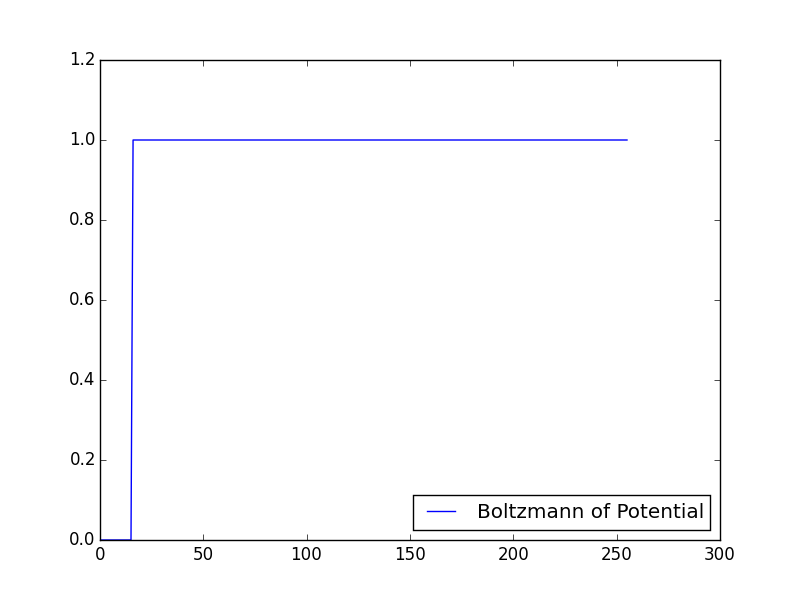
\includegraphics[width=6cm]{rdfHS2P.png}
\end{minipage}
\hfill
\begin{minipage}[hbt]{5cm}
	\centering
	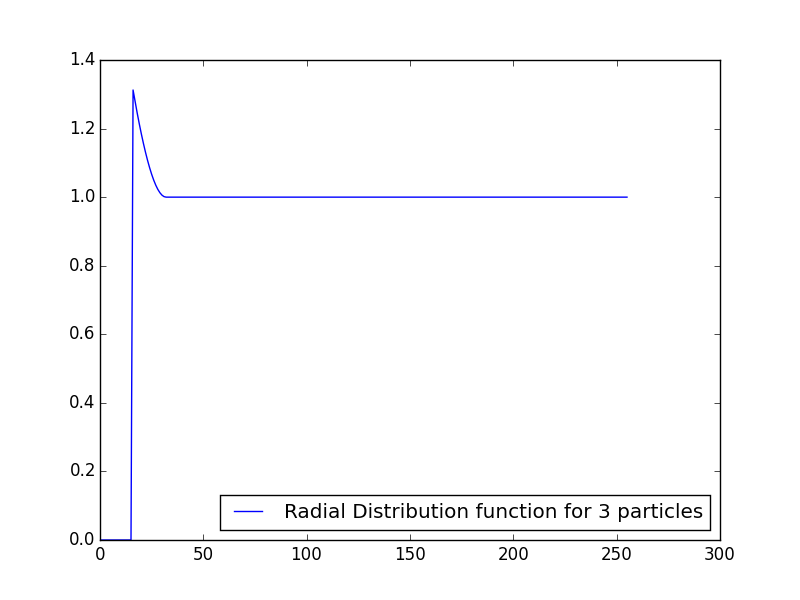
\includegraphics[width=6cm]{rdfHS3P.png}
\end{minipage}
\newline
\textit{Radial distribution function for a system comprising 2 and 3 hard sphere particles. 
One can see how a third particle affects the mutual positions between a pair of particles. 
This is amazing, since their are no (long-ranging) forces between particles, such that intuitively one could
guess that adding a third particle has no influence on the mutual separation probability. 
However, if the Volume of integration goes to infinity, the bump goes to zero, as one can expect. \newline
The convolution integral can be calculated analytically by evaluating the intersection volume of two spheres.
}
\newpage
\subsection{RDF Plots for 3 Lennard-Jones particles }
\begin{figure}[htb]
\centering
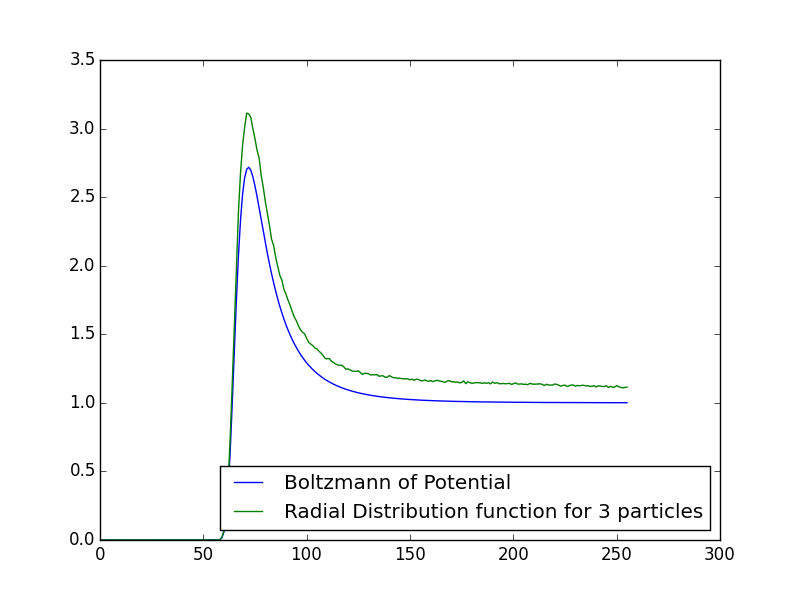
\includegraphics[width=8cm]{rdfLJ3P.png}
%\caption{Bildunterschrift}
\end{figure}
\textit{Radial distribution function for a system comprising 2 and 3 hard sphere particles for the Lennard Jones potential.
The effect of the third particle is the same as for hard spheres: The probability to find the particles at the nearest
neighbour distance increases, this can be explained by the third particle 'squeezing' the remaining two. The typical long-ranging
oscillations can't be seen for three particles only. \newline The convolution was evaluated using MC integration, this explains
the small jitter at the tail.}


\subsection{Thermodynamical constraints }
The large number of possible Bridge functions may raise the impression that there is some arbitrariness in
the resulting RDF. However, there are various thermodynamical constraints which must be fulfilled by 
$g(r)$ and hence implicitly also by the bridge function $B(r)$. We only give a simple example here to make
the principle clear. \newline
The internal energy $U$ of a liquid is given by its thermodynamical expectation value of the Hamiltonian $H$
of the system
\begin{equation}
U = \langle H \rangle = \langle T + U  \rangle
=
\langle T \rangle + \langle U  \rangle =
U_{id} + U_{ex} 
\end{equation}

where the excess internal energy is defined to be the deviation of the liquid internal energy from the ideal gas energy. 
(The ideal gas is interaction-free and hence only contains kinetic energy $\langle T \rangle$). The excess energy
in the canonical ensemble equals


\begin{equation}
U_{ex} = 
\frac{3}{2}
N(N-1) \frac{1}{Z_N}
\int u(\vec r_1, \vec r_2) 
e^{-\beta U(\vec r_1, \vec r_2, \vec r_3,\dots \vec r_n)} d\vec r_1 d\vec r_2 d\vec r_3 \dots d\vec r_n
\end{equation}

where we have chosen the particles 1 and 2 to be representative for the contribution of all the $N(N-1)$ pairs. This
allows us to integrate over particle coordinates $>2$, and we basically recover the RDF 
\begin{equation}
U_{ex} = \frac{3}{2}
\rho^2 \int u(\vec r_1, \vec r_2) g(\vec r_1, \vec r_2) d\vec r_1 d\vec r_2
=
\frac{3}{2}
\rho^2 \int u(\vec r) g(\vec r) d\vec r \int d\vec r_2
\end{equation}

where $u = u(\vec r_1 - \vec r_2)$ was used (as for $g$). Hence
\begin{equation}
U_{ex} = \frac{3}{2}
\rho^2 V \int u(\vec r) g(\vec r) d\vec r 
=
\frac{3}{2}
\rho N \int u(\vec r) g(\vec r) d\vec r
\end{equation}

such that the internal excess energy per particle is
\begin{equation}
\frac{U_{ex}}{N} = \frac{3}{2}
\rho  \int u(\vec r) g(\vec r) d\vec r
=
\frac{3}{2}\frac{4 \pi}{3}\rho  \int u(r) g(r) r^2 d r
=
2 \pi \rho  \int u(r) g(r) r^2 d r
\end{equation}

The integral in the above result matches the expectation value of the potential energy between two particles. 
(The probability to find a particle at a distance $r$ from the test particle is $g(r) r^2 d r$). \newline
The excess energy of a liquid is something which can be determined experimentally or calculated by other routes,
hence the above equation imposes a physical constraint on $g(\vec r) $. Obviously there are many functions which are compliant with this constraint, 
but at least we have a hint that something went wrong if there is a deviation from thermodynamics. \newline
As a specific example for two routes (also implemented in code, \texttt{optimizeRYalpha}, we consider the isothermal
compressibility $\kappa_T$ which can be calculated via the virial or compressibility route. The isothermal comressibility
is defined as
\begin{equation}
\kappa_T = - \frac{1}{V} \bigg( \frac{\partial V}{\partial p}\bigg)_T = 
\frac{1}{\rho} \bigg( \frac{\partial \rho}{\partial p}\bigg)_T =
\frac{1}{\rho} \bigg( \frac{\partial p}{\partial \rho} \bigg)_T^{-1}
\end{equation}

Without proof, we claim that
\begin{equation}
\kappa_T = \kappa_{T, id} \lim_{q \rightarrow 0} S_c(q) = \kappa_{T, id} \frac{1}{1 - \rho \hat c(0)}
\end{equation}
where $\kappa_{T, id}$ is the compressibility of an ideal gas which satisfies $p= \rho \beta^{-1}$ such that $\partial p/\partial \rho = \beta^{-1}$
and $\rho^{-1}(\partial p/\partial \rho)^{-1} = \beta/\rho = \kappa_{T, id}$. Hence


\begin{equation}
\kappa_T = \frac{\beta}{\rho} [1 - \rho \hat c(0)]^{-1}  \quad
\hat c(0) = 4\pi \int_{0}^{\infty} c(r) r^2 dr 
\end{equation}

For the virial route we use the pressure equation

\begin{equation}
p = p_{id} - \frac{2\pi}{3} \rho^2 I(\rho) \quad
I(\rho) = \int_{0}^{\infty} g(r; \rho) u'(r) r^3 dr
\end{equation}
such that 
\begin{equation}
\kappa_T = 
\frac{1}{\rho} \bigg( \frac{\partial p}{\partial \rho} \bigg)_T^{-1} =
\frac{1}{\rho} [\beta^{-1} - \frac{2\pi}{3} \frac{\partial}{\partial \rho}  \rho^2  I]^{-1} =
\frac{\beta}{\rho} [1 - \frac{4\pi}{3} \rho \beta I - \frac{2\pi}{3} \beta \rho^2  \frac{\partial}{\partial \rho} I ]^{-1} 
\end{equation}

comparing the two results for the compressibility we see that

\begin{equation}
\rho 4\pi \int_{0}^{\infty} c(r) r^2 dr =
\frac{4\pi}{3} \rho \beta I(\rho) +
\frac{2\pi}{3} \beta \rho^2 \frac{\partial}{\partial \rho} I(\rho)
\end{equation}

e.g. for the Lennard Jones Potential
\begin{equation}
I(\rho) =
4 \epsilon \int_{0}^{\infty} g(r; \rho) \{6(\sigma/r)^6 - 12(\sigma/r)^{12} \} r^2 dr
\end{equation}

Note that $\epsilon \beta$ is the binding energy in $k_BT$ units (dimensionless). For the Rogers Young switching function $f(r) = 1 - e^{-\alpha r}$
which tries to interpolate between PY and HNC closure via $\alpha$, both $g$ and $c$ will implicitly depend on $\alpha$. Hence we are looking
for a $\alpha^{*}$ which satisfies the thermodynamic consistency in the form
\begin{equation}
I_c(\alpha^{*}) := 4 \pi\int_{0}^{\infty} c(r; \alpha^{*}) r^2 dr =
\frac{4\pi}{3} \beta I( \alpha^{*}) +
\frac{2\pi}{3} \beta \rho \frac{\partial}{\partial \rho} I(\rho;\alpha^{*})
=: I_g(\alpha^{*})
\end{equation}
This yields yet another fixpoint problem. (But this time one dimensional). $\partial \rho I$ must be treated numerically.




\subsection{Analytical OZ solution (Unit Test)}
For hard sphere particles and the PY closure there is an analytical solution for the direct contribution function
$c(r)$. The direct contribution is assumed to be zero for $r$ larger than the hard sphere diameter
$\sigma$, since in this distance range the particles don't 'feel' each other. 
\footnote{Indirectly they do, imagine a third particle trying to slip between two others, this will be felt by the
first two, even if they are separated by a distance larger than $ \sigma$, hence $h(r > \sigma) \ne 0$}
For $r < \sigma$, there is

\begin{equation}
c(r) =
\frac{
6 \rho_V (1 + 0.5\rho_V)^2 (r/\sigma) - (1 + 2\rho_V)^2 (1 + 0.5\rho_V(r/\sigma)^3) 
}
{ (1 - \rho_V)^4 }
\end{equation}

where $\rho_V$ is the volume density of the fluid. \footnote{Not the particle number density $\rho$. $\rho_V$ is also called the 'packing fraction' or
'volume fraction'.}
The derivation can be found in Hansen and McDonald \cite{hansen2006theory}, appendix D. The pair correlation $g(r)$ can be calculated as for the fixpoint
problem. (First calculate $\Gamma$ according equation (53) and (54), then g = $\Gamma + c +1$). \newline
This solution can be used to cross check against the numerical solution. (See \texttt{PicardOZ.py} in the SciComp Git repository).

\newpage
Another 'unit test' was done by manually aligning a \texttt{SASfit} plot with the corresponding \texttt{PicardOZ.py} plot
of the structure factor $S(q)$ of a hard sphere liquid of density 0.3 and PY closure. The aligning was done by making 
the \texttt{PicardOZ.py} plot transparent and overlaying it to the \texttt{SASfit} plot in a way that the axes are adjusted. 
The two plots coincidence to a high degree


\begin{figure}[htb]
\centering
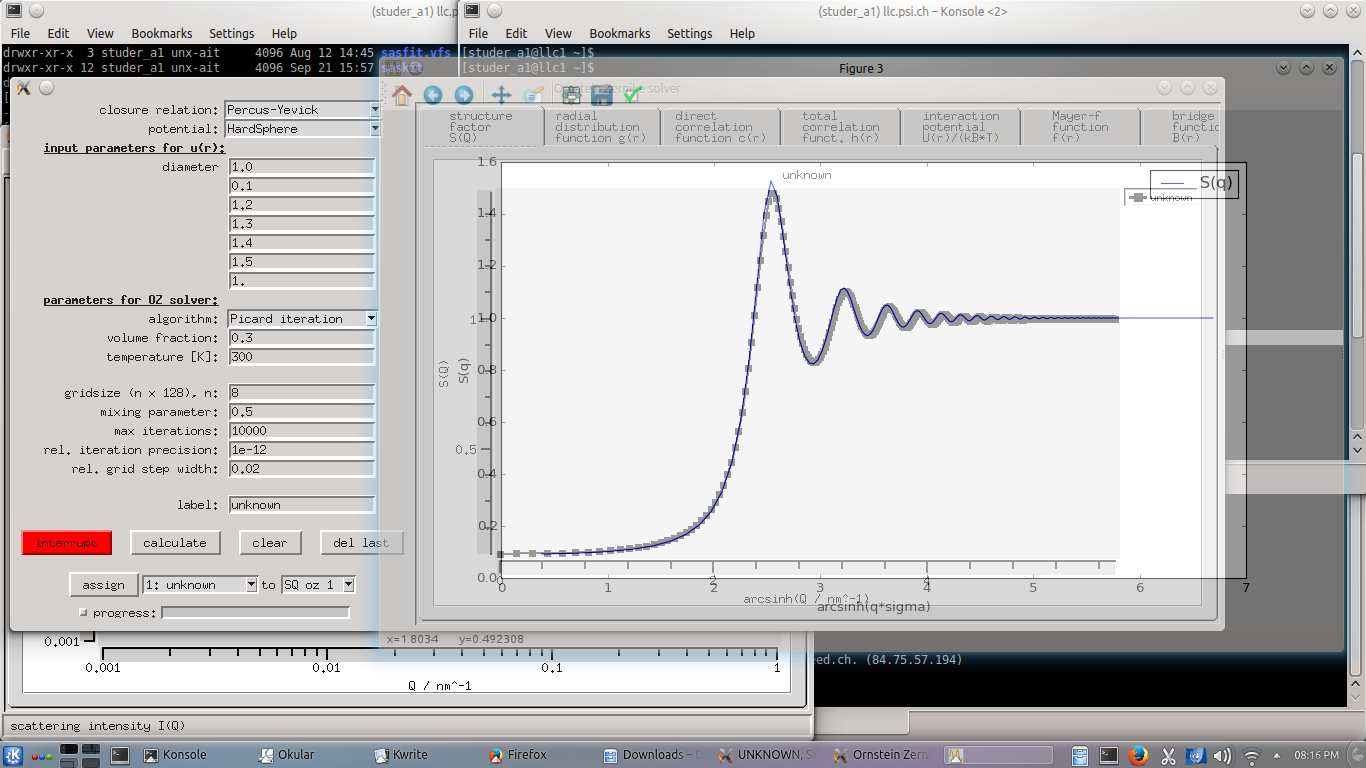
\includegraphics[width=12cm]{PyOZ-SASfit_SqHS03PY.png}
%\caption{Bildunterschrift}
\end{figure}
\textit{Structure factor plots for a hard sphere liquid of density 0.3 and PY closure. The blue curve is the result of the
python code whereas the black square-dotted curve is the result of the reference SASfit code. The differing 'triangle' on top may be
a consequence of the plot rendering mode. Furthermore, the two coordinate systems could not be aligned perfectly. \newline
The  \texttt{arcsinh} scale of the \texttt{q} axis is just for visibility, in order to plot the structure factor S($\theta$)
as a function of the scattering angle $\theta$, \texttt{arcsin} scaling would be adequate. }



\subsection{Sources}
Some information and illustrations were taken from \href{https://en.wikipedia.org/wiki/Radial_distribution_function}{Wikipedia}.
For me the simple but intuitive derivation of the closure relations were helpful. 
(See e.g. \href{https://en.wikipedia.org/wiki/Percus%E2%80%93Yevick_approximation}{PY})
\newline
Most of the theory was taken from the book of Hansen and McDonald \cite{hansen2006theory} which can be downloaded
from the internet \href{http://www.sciencedirect.com/science/book/9780123705358}{here}. 
\newline
\texttt{SASfit} specific information can be found on the  
\href{http://sourceforge.net/p/sasfit/sasfit/ci/tip/tree/doc/manual/sasfit.pdf}{project sourceforge site}.
\newline
A standalone version of AAA (outside OZ scope) can be found on 
\href{https://gitorious.psi.ch/scicomp/aa4oz/trees/master/src}{SciComp Git repository}. There you can also find 
the python scripts used to calculate the three-particle RDF.
\newline
AAA for OZ is located in the project
\href{http://sourceforge.net/p/sasfit/sasfit/ci/tip/tree/src/sasfit_oz/sasfit_oz_solver.c}{source file},
starting from the corresponding case statement ($\simeq$ line 1212).

\subsection{Potential design improvement for SASfit}
Observing the first method of the \texttt{OZ\_solver.c} file reveals that the MVC pattern might be violated. 
\lstset{language=C}
\begin{lstlisting}[frame=single]  
#define GET_TCL(val_type, target, src_name) 
(sasfit_tcl_get_ ## val_type(interp, target, \
ozname, src_name) == TCL_OK)

void check_interrupt(sasfit_oz_data *OZd) {
 int interupt_signal;
 Tcl_Interp *interp;
 char * ozname = Tcl_GetStringFromObj(OZd->oz_obj, 0);

 interp = OZd->interp;
 if (!GET_TCL(int, &OZd->PrintProgress, 
           "PrintProgress")) {
            OZd->PrintProgress = 0;
    }
........................................
}
\end{lstlisting}
The \texttt{OZ\_solver.c} module is responsible for solving the OZ equation and as such it should be fully agnostic about
the GUI implementation to which it is connected. The cleanest way to separate GUI and solver is by running them 
as different processes. Seen from a GUI-independent level of abstraction, the only interaction between
the (GUI-)client and the solver consists of the mutual information start, stop, interrupt, continue, finished. In the Unix world, a generic way
to implement this (inter-process) communication would be by POSIX compliant signals. The OZsolver (the server) would install
a signal handler for the \textit{start\_calculation}, \textit{stop\_calculation}, \textit{interrupt\_calculation}, and \textit{continue\_calculation}
signals which can be emitted by the client. Conversely, the server can send a \textit{finished\_calculation} signal if it finished (successfully) and 
hence the result is ready to be delivered in a predefined way to the client. (The result may be written to a file, shared memory or socket). 
The input parameters would be delivered to the server as well by a 'generic channel'. \newline
Implemented like this, any (GUI-)client could connect to the server without modifying and/or recompiling the OZsolver code.
Running the client in a different process has also advantages for Tcl/Tk (the current GUI implementation) due to the 
limited multi-threading capabilities of Tcl/Tk. \newline
Since the GUI is also supposed to work on Windows systems and maybe even cross-platform and/or multinode
(e.g. the OZsolver running on a Linux cluster controlled by a GUI process running on Windows), the IPC is best implemented on top of TCP/IP. 
%(E.g as a Browser plus REST interface)
\newpage
As a proof of concept, these ideas are implemented using remote procedure calls. (Code is in \texttt{./src/RPC} directory on gitorious).
\newline Summary/description of the code: Server side, one can start as many OZsolver processes as desirable 
(typically as many as there are cores on the server machine).
The OZsolver class (whose instance basically constitutes a OZsolver process) exposes its getter and setter methods via a RPC interface
which can be called from the client process. The client process typically sets up a range of parameters to be scanned, e.g a range of density parameters.
These parameters are then set via the RPC setter method \texttt{setVolumeDensity} and 
subsequently the (remote) \texttt{solve} method is called to trigger the calculation on the servicing process.
Finally, the results are collected by the client using \texttt{getRDFasList} method. (The results are sent over the network if the client runs on
a different machine than the server). \newline 
The RPC protocol is \texttt{http} based, so there is some runtime and communication overhead, but benchmarks show that the application
scales well with the number of cores (processes).


\subsection{Getting and Compiling SASfit code}
Project has moved to GitHub
\lstset{language=bash}
\begin{lstlisting}[frame=single]  
$ git clone https://github.com/SASfit/SASfit.git
$ cd SASfit
$ mkdir build
$ cd build/
*******************************************
SL6 cmake is outdated for this purpose, 
install cmake >= 3.3
$ /home/studer_a1/cmake/bin/cmake --version
*******************************************
$ $HOME/cmake/bin/cmake ../src #configure
*******************************************
On Unix machine, you can add option
-G "Unix Makefiles"
*******************************************
$ make #compile
$ ../sasfit #run
\end{lstlisting}
This works on \texttt{llc.psi.ch} machines, but since these are 32 bit, make sure to compile the up to date \texttt{cmake} also on a \texttt{llc} machine.
\newpage
\bibliographystyle{plain}       % or "unsrt", "alpha", "abbrv", etc.
\bibliography{FPC}           % use data in file "FPC.bib"
\end{document}
